\chapter{Replication and Extension}

\section{Introduction}

In the previous chapter, we have seen the results of applying my proposed model inference technique on the data collected from our industry partner, MicroPilot. However, to confirm the results and idea furthermore a second study on a similar software is quite helpful. 
In this chapter I present the process and the results of replicating that paper on Paparazzi, an open source equivalent to MicroPilot's auto-pilot.
In the second case study in addition to confirming that the technique is applicable on other software, I could improve on some aspects as well.
I could replicate the relative differences in performance of different CPD methods. The same goes with classic machine learning classifiers: a linear classifier with regularization and a decision tree classifier. 
Also, I confirmed that a similar neural network architecture can be trained to infer an state model of Paparazzi as well.

In addition to replicating these, I created a hyper-parameter tuning pipeline to get a better performance out of the neural network model. I used a simple grid search technique over the hyper-parameters, in two steps to find the sweet spot for the best overall performance as measured by 8 metrics.
The result of this tuning was a model with fewer convolutional layers and smaller kernel sizes but with more convolutional filters and recurrent layers that could perform better than the baselines. This shows having more and smaller convolutional filters is more effective in capturing local features in the data compared to having a small number of large filters (with kernels of size 20 for example which has 200 parameters). It also shows the important role that recurrent layers play in discovering long-term relations between inputs and outputs. 


\section{The Case Study Subject}
I chose Paparazzi auto pilot as an open-source alternative to MP\footnote{MicroPilot}'s auto-pilot for replication. Paparazzi \cite{hattenberger2014using} project started in 2003 as an academic auto-pilot and continues to be developed with the state of the art in the autonomous flying vehicle's field. Another major player in open source auto-pilot software scene is ArduPlane; however I chose to do this study only on Paparazzi for the following reasons:
A comparison about how Paparazzi is superior to ArduPlane can be read at \url{https://wiki.paparazziuav.org/wiki/Paparazzi_vs_X}. 
In addition to that, after doing a preliminary study, I found out that Paparazzi has a more straightforward and robust protocol for remote controlling and data collection, as explained previously in section~\ref{sec:paparazzi_data_collection}. 
Furthermore, Paparazzi supports multiple flight dynamic model (FDM) simulators. One of them is JBSim\footnote{\url{http://jsbsim.sourceforge.net/}} which provides an advanced physical model of complex dynamics in air-frames and sensors for an accurate and close to the reality simulation. 


\section{Objectives}
\subsection{RQ 1) Can the results be replicated with regards to state change point detection (CPD)?}
I ran 42 different combinations of settings for CPD algorithms in ``ruptures'' library \cite{Truong2018ChangePointSurvey}. 
There are 7 cost functions, 3 search methods (1 exact and 2 approximate), and 3 penalty values (100, 500, and 1000).
I used the same configurations in the previous study. 
To evaluate them, I used the same precision, recall, and F1 score (with a margin of tolerance) as the previous study which are defined in section~\ref{sec:CPD_metrics}.

\subsection{RQ 2) Can the results be replicated with regards to internal state prediction?}
I fed the data to a number of classic machine learning algorithms as baselines. The problem setting is a multi-class classification, though with Paparazzi the number of classes are smaller. 
There are 20 possible states in Paparazzi as opposed to MicroPilot's 25. This is due to their differences in solving the problem of defining a mission and controlling an automated vehicle (the aircraft) to perform it.

\subsection{RQ 3) How will hyper-parameter tuning affect the results?}
In previous study the hyper-parameters of the neural network model were tuned manually. Hyper-parameters include the number of convolutional layers, number of convolutional filters in each layer, number of recurrent cells, and optimizer parameters such as learning rate. There are no gold standards for the values of these parameters, they need to be tuned for each problem. In the replication I opted for existing automated ways for finding better hyper-parameters.

The training data was split into 3 chunks after shuffling: 70\% of the data was used for training, 20\% was used as the test set for tuning the hyper-parameters, and the remaining 10\% was set aside as the validation data to measure the trained model's performance. 


\section{Experiment}
\subsection{Data Collection}
The process of collecting the data has already been explained in chapter~\ref{chapter:fuzz_tester} in detail. However, let us have a quick recapitulation:
Unlike MP, Paparazzi did not include any system tests. So, I developed a fuzz tester tool to generate valid, diverse, and meaningful test plans based on the example flight plan that is shipped with the software. My tool can automatically generate system tests, run them in a simulator (or on hardware\footnote{Although I have not tested running tests on a hardware (HWIL, see section~\ref{sec:mp_test_scenarios}) to confirm, but having implemented the protocol it potentially is capable of doing so}), and also collect required telemetry data from the aircraft. The targeted randomizations in test inputs are augmented with the stochastic wind model in the simulation to further diversify the observed behaviours. My fuzz tester tool ran ran each generated scenario in a simulation and recorded the required flight data.
The result was 378 runs worth of different flight scenarios.
After collecting the data I performed some pre-processing steps on them to make them more similar to what the previous model was trained on. These pre-processing steps include normalizing some values as well as metric to imperial unit conversions.

Figure~\ref{fig:paparazzi_test_length} shows the distribution of test lengths. The test lengths range from 140 samples (70 seconds) to 2580 samples, with a median of 2170 and a mean of 1896.
\begin{figure}
    \centering
    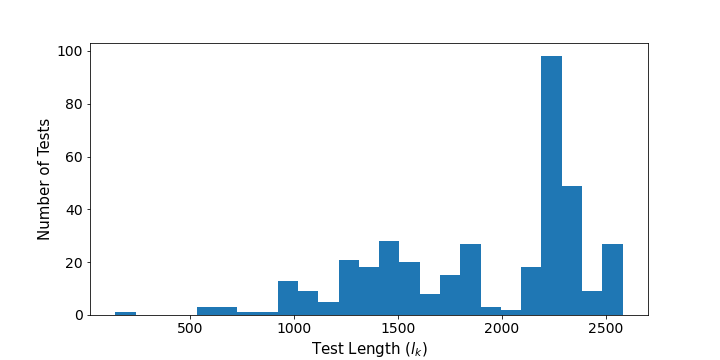
\includegraphics[width=\columnwidth]{6_files/test_lengths.png}
    \caption{The histogram of number of tests of different test sizes. The smallest samples contains 140 samples worth of recorded flight data and the largest one has 2580 samples, equivalent of a 516-second flight (Sampling rate is 5Hz). }
    \label{fig:paparazzi_test_length}
\end{figure}


\subsection{CPD baselines (RQ 1)}
Similar to the MicroPilot study, I fed the data from Paparazzi to several CPD baselines implemented in ``ruptures'' library.
Fortunately, with smaller data set size (in comparison to MP's), it was feasible (though still time-consuming) to try ``Pelt'' CPD method \cite{killick2012optimal} as well, making the replication study is richer in that sense. Pelt is the most efficient exact CPD method which, as mentioned before, failed to scale up to process MP's data. All other CPD methods are approximate algorithms.

\subsection{Classification algorithms (RQ 2)}
I used a ridge classifier and a decision tree classifier with 3 settings for maximum number of features with no limit on their depths. This setting is the same as the MP's case, with the only difference being on removing the depth limit. Tuning the depth limit was an arduous and inaccurate task that resulted in minimal improvements (if any), so it was not worth the time. Overall, I ran $(1+3)\times6=24$ different settings for classic learning algorithms. 

\subsection{Hyper-parameter Tuning (RQ 3)}
I created a model creation and evaluation pipeline that takes hyper-parameters as the input and outputs the model performance scores on test data as its output. The hyper-parameters that I searched over are:
\begin{itemize}
    \item Number of GRU cells in the recurrent section: between 32 and 256
    \item Number of convolutional filters in each layer: between 16 to 64
    \item The size of convolution kernels and the number of convolutional layers: between 3 to 5 layers with increasing kernel size
    \item The learning rate of Adam optimizer: from $1\times 10^{-4}$ to $3\times10^{-3}$
\end{itemize}
Please refer to figure~\ref{fig:model_arch} for a recap on these hyper-parameters. 
I performed an exhaustive grid search over these parameters, using Tensor Board for keeping track of the metrics and finding the right balance.

Tensor Board is a monitoring tool made for TensorFlow \cite{tensorflow2015-whitepaper} that provides great insight for better training TensorFlow models.

\section{Results}
\subsection{CPD baselines (RQ 1)}

The results of applying baseline algorithms on Paparazzi data set can be seen in table~\ref{tab:cpd_paparazzi}.
The numbers are quite varied, there are scores worse then 1\% as well as some 100\% recall scores. The 100\% recalls are accompanied with a low precision; achieving that is not difficult. A method that outputs every point as a change-point will get similar results. The setting that got most of the best numbers is Pelt algorithm using an L1 cost function and a high penalty coefficient of 1000. However, please note that Pelt is a quite slow algorithm that could easily become infeasible to run on larger data set, as it was the case for MP's study. As a matter of fact, in this study getting the results for Pelt took more than 14 hours on the same machine that performed all other CPD algorithms in less than 1 hour. What you see in table~\ref{tab:cpd_paparazzi} is the summary of the results of more than 23800 experiments. 

Comparing the baseline results with the neural network model's results in the last three rows of the table, you can see improvements of 48.9\%, 26.83\%, and 11.46\% in F1 scores compared to the best numbers in the baselines (for $\tau = 1, 3, 5$ seconds respectively). Although this model still performed better than the baselines, the improvement margin was higher in the MP study (See the RQ1 results summary box and the paragraph above that in section~\ref{sec:results}). However, you can see that the scores that this approach achieved are not low, but the baselines could do a better job on Paparazzi's data compared to MicroPilot's, therefore shrinking the margin of improvement. It can be due to the fact that the new data set is tiny compared to MP, classic machine learning algorithms can do better so a deep learning model cannot shine here as it could for MP. To reiterate, Paparazzi data set consists of ~300 tests vs. ~900 tests in MP, and simulation lengths are up to 2500 samples vs. 18000 sample tests in MP's data set. It is worth mentioning that both in the original study on MP's data and here, the variation in baselines performances was way higher while my deep learning approach shows a more consistent performance; check the second column (recall with $\tau=1$s) for example. 

\begin{sidewaystable}
    \centering
\resizebox{\columnwidth}{!}{%
\begin{tabular}{llcccccccccc}
\toprule
  \textbf{Cost Function} &
  \textbf{Search Method} &
  \textbf{Penalty} &
  \textbf{Prec.} &
  \textbf{Recall} &
  \textbf{F1} &
  \textbf{Prec.} &
  \textbf{Recall} &
  \textbf{F1} &
  \textbf{Prec.} &
  \textbf{Recall} &
  \textbf{F1} \\
                                                  &              &   & \multicolumn{3}{c}{$\tau=1$s} & \multicolumn{3}{c}{$\tau=3$s} & \multicolumn{3}{c}{$\tau=5$s} \\  \toprule
\multirow{3}{*}{\textbf{Autoregressive Model}}
    & bottomup & 500  &       13.65\% &    14.13\% & 18.89\% &        39.73\% &     36.40\% & 36.14\% &        57.11\% &     53.20\% & 50.04\% \\
    & exact & 500  &       13.56\% &    13.85\% & 19.03\% &        39.67\% &     36.17\% & 36.03\% &        56.97\% &     52.89\% & 49.83\% \\
    & window & 100  &       15.97\% &     7.59\% & 13.54\% &        45.47\% &     20.40\% & 29.56\% &        64.16\% &     30.76\% & 41.20\% \\ \midrule
\multirow{3}{*}{\textbf{Least Absolute Deviation}}
    & window & 100  &       24.50\% &    15.92\% & 19.85\% &        56.39\% &     37.24\% & 44.53\% &        68.94\% &     48.20\% & 56.23\% \\
    & exact & 1000 &       \textbf{26.74\%} &    34.08\% & 29.92\% &        \textbf{60.77\%} &     77.32\% & \textbf{67.74\%} &        \textbf{74.73\%} &     93.16\% & \textbf{82.61\%} \\
    & bottomup & 1000 &       26.66\% &\textbf{34.99\%}& 30.35\% &        60.11\% &     78.14\% & 67.61\% &        72.85\% &     92.94\% & 81.30\% \\ \midrule
\multirow{3}{*}{\textbf{Least Squared Deviation}}
    & window & 1000 &       25.01\% &    16.14\% & 20.26\% &        54.58\% &     35.77\% & 42.96\% &        68.73\% &     48.11\% & 56.18\% \\
    & exact & 1000 &       21.28\% &    80.04\% & 33.49\% &        51.05\% &     99.58\% & 67.20\% &        65.36\% & \textbf{99.97\%} & 78.76\% \\
    & bottomup & 1000 &       21.30\% &    81.24\% & \textbf{33.62\%} &        50.98\% &\textbf{99.50\%}& 67.12\% &        65.24\% &\textbf{99.97\%}& 78.66\% \\ \midrule
\multirow{3}{*}{\textbf{Linear Model Change}}
    & bottomup & 100  &        7.39\% &     0.39\% &  9.98\% &        27.44\% &      1.49\% & 10.27\% &        52.51\% &      2.75\% &  9.90\% \\
    & window & 100  &        7.39\% &     0.39\% &  9.98\% &        27.44\% &      1.49\% & 10.27\% &        52.51\% &      2.75\% &  9.90\% \\
    & exact & 100  &        7.39\% &     0.39\% &  9.98\% &        27.44\% &      1.49\% & 10.27\% &        52.51\% &      2.75\% &  9.90\% \\ \midrule
\multirow{3}{*}{\textbf{Gaussian Process Change}}
    & window & 100  &        7.39\% &     0.39\% &  9.98\% &        27.44\% &      1.49\% & 10.27\% &        52.51\% &      2.75\% &  9.90\% \\
    & exact & 100  &        7.39\% &     0.39\% &  9.98\% &        27.44\% &      1.49\% & 10.27\% &        52.51\% &      2.75\% &  9.90\% \\
    & bottomup & 100  &       12.42\% &   \textbf{100.00\%} & 22.03\% &        33.15\% &    \textbf{100.00\%} & 49.55\% &        49.04\% &    \textbf{100.00\%} & 65.47\% \\ \midrule
\multirow{2}{*}{\textbf{Rank-based Cost Function}}
    & exact & 100  &       21.11\% &    31.85\% & 25.51\% &        52.29\% &     74.63\% & 61.13\% &        65.88\% &     89.30\% & 75.46\% \\
    & bottomup & 100  &       20.55\% &    31.84\% & 25.17\% &        49.97\% &     73.22\% & 59.04\% &        64.57\% &     89.35\% & 74.61\% \\ \midrule
\multirow{3}{*}{\textbf{Kernelized Mean Change}} 
    & bottomup & 100  &       15.66\% &     1.90\% &  9.45\% &        44.23\% &      5.36\% & 12.95\% &        62.37\% &      7.48\% & 15.66\% \\
    & exact & 100  &       14.07\% &     1.64\% &  9.77\% &        42.06\% &      4.74\% & 12.59\% &        60.92\% &      6.67\% & 14.56\% \\
    & window & 100  &        8.31\% &     0.61\% &  9.97\% &        29.38\% &      2.02\% & 10.60\% &        53.34\% &      3.39\% & 10.79\% \\ \midrule \midrule
\multirow{3}{*}{\textbf{My approach}} 
    & \multirow{3}{*}{\textbf{Data set:}}  
         & \textbf{Validation} &  45.63\% &    55.46\% & 50.07\% &   81.39\% &     90.97\% & 85.92\% &   88.38\% &     97.12\% & 92.54\%  \\
    & {} & b\textbf{Test (Tuning)} &  42.65\% &    54.87\% & 47.99\% &   76.73\% &     90.96\% & 83.24\% &   85.18\% &     97.46\% & 90.91\%  \\
    & {} & \textbf{Training}  &  39.81\% &    51.96\% & 45.08\% &   75.69\% &     90.62\% & 82.49\% &   84.96\% &     97.55\% & 90.82\%  \\
\bottomrule
\end{tabular}%
}
    \caption{Change point detection methods performance on Paparazzi data set. Since the 100\% recalls are actually outliers, the next largest recall values are in bold face as well.}
    \label{tab:cpd_paparazzi}
\end{sidewaystable}

\subsection{Classification algorithms (RQ 2)}
In table~\ref{tab:rq2-1-results-replicate} the comparative results of the aforementioned algorithms with my method is presented. 
To compare with the original study, we can see that in all but two settings limiting the maximum number of features did not help improve the model. Another similar observation is that the scores do not vary very much with changing the window size, and decision trees almost universally outperform linear classifiers.
The scores themselves are just around the same values as well: Ridge classifier F1 score here is in 21-29\% which was 32-39\% in the original study, for decision trees it is in 67-68\% here and it was 73-77\% in the original study. 

The deep learning model's performance measures (on validation data) can be found in the last row of the table. 
You can see an $(81.92-68.96)-1=18.79\%$ improvement in F1 score, over the baselines. It confirms that this method can beat the best performing baselines in classifying input samples into the system's internal states. The improvement in the original study was 16.83\%. This, again confirms the reproducibility of the results from 

\begin{table}
\caption{Precision, recall, and F1 score of ridge classifiers (linear classifiers with L2 regularization) and decision tree classifiers with different sliding window widths ($w$). In this table, we only show the results of the best performing model in each group.}
\label{tab:rq2-1-results-replicate}
\resizebox{\linewidth}{!}{%
\begin{tabular}{llcccc}
\toprule
\textbf{w} &
  \multicolumn{1}{c}{\textbf{Classifier}} &
  \multicolumn{1}{c}{\textbf{Max Features}} &
  \multicolumn{1}{c}{\textbf{Precision}} &
  \multicolumn{1}{c}{\textbf{Recall}} &
  \multicolumn{1}{c}{\textbf{F1}} \\ \midrule
 3 &  Ridge &            - &      44.82\% &   14.45\% & 21.85\% \\
 3 & Decision Tree & $\sqrt{10w}$ &      61.88\% &   73.56\% & 67.22\% \\ \midrule
 5 &  Ridge &            - &      46.62\% &   15.10\% & 22.81\% \\
 5 & Decision Tree &            - &      64.28\% &   73.00\% & 68.36\% \\ \midrule
10 &  Ridge &            - &      47.59\% &   16.29\% & 24.27\% \\
10 & Decision Tree &            - &\textbf{65.06\%}& 73.36\% &\textbf{68.96\%}\\ \midrule
15 &  Ridge &            - &      44.41\% &   17.33\% & 24.93\% \\
15 & Decision Tree &            - &      63.53\% &   74.68\%& 68.65\% \\ \midrule
20 &  Ridge &            - &      57.97\% &   19.10\% & 28.74\% \\
20 & Decision Tree &            - &      64.72\% &   73.36\% & 68.77\% \\ \midrule
25 &  Ridge &            - &      62.13\% &   19.66\% & 29.87\% \\
25 & Decision Tree & $\sqrt{10w}$ &      61.17\% &\textbf{75.18}\% & 67.45\% \\ \midrule \midrule
   & \multicolumn{2}{l}{Proposed Method} & \textbf{71.13\%} & \textbf{88.69\%} & \textbf{81.92\%} \\
\bottomrule
\end{tabular}%
}
\end{table}

They say a picture is worth a thousand words\footnote{missing citation}, to better see the predictions of the deep learning model compared to the ground truth, see figure~\ref{fig:paparazzi_predictions}. 
\begin{figure}
    \centering
    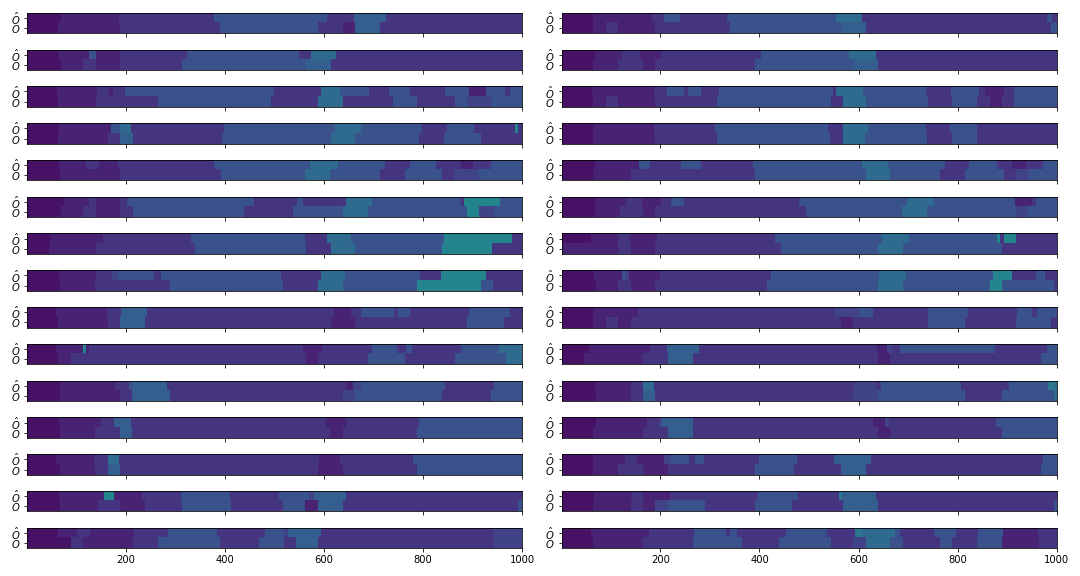
\includegraphics[width=\columnwidth]{6_files/states_chart.png}
    \caption{The states are color coded and each rectangle shows one test, only the first 1000 samples (200 seconds) are shown for more clarity. The same as figure~\ref{fig:test_0} in the previous chapter, the top half of each rectangle shows the model's output and the bottom half shows the true labels.}
    \label{fig:paparazzi_predictions}
\end{figure}

\subsection{Hyper-parameter Tuning (RQ 3)}
I used Tensor Board to visualize and compare the effects of different hyper-parameters on the model's performance. First, for a sanity check, I visualized 4 metrics, precision and recall in detecting change points with a small tolerance of $\tau=1s$, and precision and recall in estimating the internal state. A healthy linear and positive correlation is visible between all pairs of these metrics, it means that trying to improve one usually will not come at the expense of others. 
\begin{figure}
    \centering
    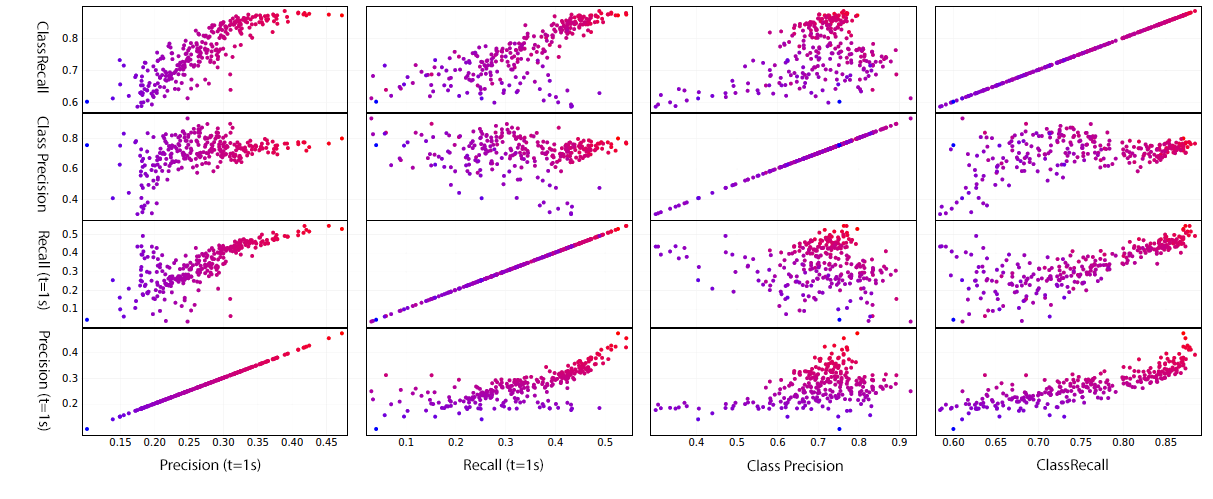
\includegraphics[width=\columnwidth]{6_files/prec_recall_matrix_tuning_white_background.png}
    \caption{Matrix of scatter plots comparing precision and recall of the deep learning model on test data.}
    \label{fig:precision_recall_matrix}
\end{figure}

Filtering the data to find the commonalities of better hyper-parameters shows that the number of GRU cells has a high correlation with both CPD precision and classification precision. 
It also shows that the kernel sizes and number of convolutional layers does not have an as strong correlation with higher precision and recalls. The number of convolutional filters in each layer has a bigger impact on the performance than the size of the kernels does. 
It makes sense because training larger kernels gets harder and harder and requires more data. Also, based on the previous studies, especially in the field of computer vision, we can say that each filter learns one feature so it is more effective to have many small filters that are easier to train and can learn multiple features of the data.
Therefore we can reduce the size of convolutional section of the model and use more recurrent cells to boost the performance without adding too many parameters. I performed another set of tests in a smaller search space to further optimize the hyper-parameters.

The new search space was all the combinations of these hyper-parameters:

\begin{enumerate}
    \item Learning rate, options being: $3\times10^{-4}$, $1\times10^{-3}$, and $3\times10^{-3}$
    \item Number of GRU cells, options: 128, 256, 384, and 512
    \item Number of convolutional filters in each layer: 32, 64, and 72
\end{enumerate}

\begin{figure}
    \centering
    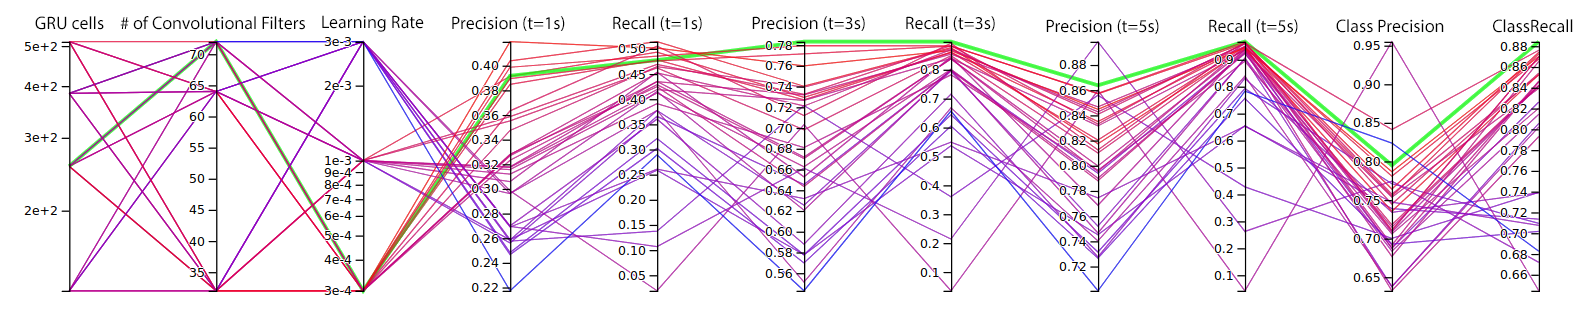
\includegraphics[width=\columnwidth]{6_files/refined_prec_recall_white_background.png}
    \caption{Parallel coordinates view showing the effects of select hyper-parameters on the performance measures.}
    \label{fig:precision_recall_parallel_coordinates}
\end{figure}
The results of the second round of tuning are shown in figure~\ref{fig:precision_recall_parallel_coordinates}. This chart shows 3 + 8 parallel axis, 3 hyper-parameters and 8 metrics. To make it more legible, the results with lower than 70\% precision ($\tau = 5s$) are omitted.
The green highlighted line is the best configuration tried, with the highest area under the curve. That configuration has the best or close to the best performance in all metrics. The configuration is to use 256 GRU cells, 72 filter per layer, and the lower learning rate of $3\times10^{-4}$.

I used these hyper-parameters to train the best model. The scores used in the first two research question are the evaluation results of this model on the previously unseen validation data. The stopping criteria on training the model was for the validation loss to plateau, with a `patience' of 15 epochs. The optimizer converged in 54 epochs, after less than 3 minutes of training. 
